% !TeX document-id = {162e9e21-9983-435d-9452-f8de7c260717}
% !TeX program = lualatex
% !BIB TS-program = biber
\documentclass[10pt,aspectratio=169,english]{beamer}
\usepackage{graphicx} % Required for inserting images
\usepackage{caption}
\usepackage{subcaption}
\usepackage{complexity}
\usepackage{framed}

%\usepackage[charter]{mathdesign}
% \usepackage{xcharter-otf}
% \usepackage{hologo}
% \usepackage{luamesh}

\usepackage[english]{babel}
\usepackage{tcolorbox}
\usepackage[style=authoryear, backend=biber]{biblatex}
\usepackage{cleveref}
% \hypersetup{colorlinks=true}

\usepackage{tikz}
\usetikzlibrary {graphs, graphs.standard, graphdrawing, fit, arrows.meta, positioning, calc, decorations.pathmorphing, shapes}
\usegdlibrary {layered} 
\usegdlibrary {circular}
\usegdlibrary{force}
\usegdlibrary{trees}

\pgfdeclareimage[width=6mm]{tree}{tree}
\pgfdeclareimage[width=5mm]{fire}{fire}
\pgfdeclareimage[width=6mm]{fighter}{fighter}

%\usepackage{beamerthemeAmurmaple}

\tcbuselibrary{listings,breakable}
\tcbuselibrary{documentation}
\tcbset{
  color command=AmurmapleRed,
  color environment=AmurmapleRed,
  color option=AmurmapleGreen
}

%\usepackage{cmbright}

\usetheme[
%nogauge,
nomail,
%delaunay,
%amurmapleblue
]{Amurmaple}

\lstset{
  numberstyle=\footnotesize\color{gray},
  keywordstyle=\ttfamily\bfseries\color{structure},
  basicstyle=\ttfamily\normalsize,
  commentstyle=\itshape\color{gray},
  stringstyle=\ttfamily,
  showstringspaces=false,
  language=[LaTeX]TeX,
  breaklines=true,
  breakindent=30pt,
  defaultdialect=[LaTeX]TeX,
  morekeywords={usetheme,definecolor, beamerbutton, beamerskipbutton,
    beamerreturnbutton, structure, alert, sectionpage, mail, webpage,
    collaboration, subtitle, institute, titlegraphic, sepframe, includegraphics,
    thanksframe, inserttitlegraphic, framesection, boxalert,appendix,logo}
  % frame=tb
}

\newtcblisting{Code}{%
  arc=0pt,outer arc=0pt,
  colback=structure!3,
  colframe=structure,
  breakable,
  boxsep=0pt,left=5pt,right=5pt,top=5pt,bottom=5pt, bottomtitle =
  3pt, toptitle=3pt,
  boxrule=0pt,bottomrule=0.5pt,toprule=0.5pt, toprule at break =
  0pt, bottomrule at break = 0pt,
  listing options={breaklines,basicstyle=\ttfamily},listing only,
}

\newtcblisting{Exemple}{%
  arc=0pt,outer arc=0pt,
  colback=structure!3,
  colframe=structure,
  breakable,
  boxsep=0pt,left=3pt,right=3pt,top=2pt,bottom=2pt, bottomtitle =
  0pt, toptitle=0pt,
  boxrule=0pt,bottomrule=0.5pt,toprule=0.5pt, toprule at break =
  0pt, bottomrule at break = 0pt,
  listing options={breaklines,basicstyle=\ttfamily},
}

\newtcblisting{CodePreambule}{%
  arc=0pt,outer arc=0pt,
  colback=AmurmapleBlue!5,
  colframe=AmurmapleBlue,
  breakable,
  boxsep=0pt,left=5pt,right=5pt,top=5pt,bottom=5pt, bottomtitle =
  3pt, toptitle=3pt,
  boxrule=0pt,bottomrule=0.5pt,toprule=0.5pt, toprule at break =
  0pt, bottomrule at break = 0pt,
  enhanced,
  overlay  ={%
    \node[ minimum width=1cm,
      anchor=south east,yshift=-0cm,fill=AmurmapleBlue] at (frame.south east)
      {\itshape\color{white} preamble};
      % \node[ minimum width=1cm,
      % anchor=south east,yshift=-0cm,color=gray,opacity=0.7] at (frame.south east)
      % {\itshape\small préambule};
  },
  listing options={
    breaklines,
    basicstyle=\ttfamily,
  },listing only,
}

\newtheorem{proposition}{Proposition}


\title[Restricting infections on graphs]{Restricting infections on graphs}
\author[S.~Santos]{Samuel Santos}
\subtitle{Immunization problems}
\institute[UFC]{UFC\\
Universidade Federal do Ceará}
\date{December 2024}
\titlegraphic{
\includegraphics[width=2.4cm]{ufc-logo.png}}
\mail{csamuelssm@alu.ufc.br}
%\webpage{www.ceremade.dauphine.fr/~chupin/}
\collaboration{Supervised by Ana Karolinna Maia and Carlos Vinícius G. C. Lima}

\bibliography{biblio.bib}
\usefonttheme{default}
\DeclareMathVersion{sans}
\SetSymbolFont{operators}{sans}{OT1}{cmbr}{m}{n}
\SetSymbolFont{letters}{sans}{OML}{cmbrm}{m}{it}
\SetSymbolFont{symbols}{sans}{OMS}{cmbrs}{m}{n}
\SetMathAlphabet{\mathit}{sans}{OT1}{cmbr}{m}{sl}
\SetMathAlphabet{\mathbf}{sans}{OT1}{cmbr}{bx}{n}
\SetMathAlphabet{\mathtt}{sans}{OT1}{cmtl}{m}{n}
\SetSymbolFont{largesymbols}{sans}{OMX}{iwona}{m}{n}
\sffamily\mathversion{sans}
%\renewcommand{\familydefault}{\sfdefault}
%\renewcommand{\sfdefault}{cmbr}
%\renewcommand{\ttdefault}{cmbr}
%\usefonttheme{professionalfonts}

\begin{document}

\maketitle

\section{Introduction}

\begin{frame}{Introduction}

\onslide<1->{
    Several phenomena happen in a \textbf{contagion-like manner}.
    
    \begin{minipage}{\textwidth}
    	\begin{itemize}
    		\item<1-> Viruses or bacteria;
    		\item<1-> Innovation, (mis-)information, and memes. \parencite{ryan2017acceptance, Coleman1957-tv}	
    		%\item<3-> Even bedbugs seem to spread from hotel to hotel via travelers \parencite{barabasi2016network}.
    	\end{itemize}
    \end{minipage}%\begin{minipage}{0.5\textwidth}
%	    \only<2>{
%	    	\begin{information}
%	    		{\footnotesize Studies found that most people adopt innovative ideas based on the experience of their neighbors or community.
%	    		\begin{itemize}
%	    			\item The adoption of hybrid seed corn among farmers \parencite{ryan2017acceptance};
%	    			\item The adoption of tetracycline by physicians \parencite{Coleman1957-tv}.
%	    		\end{itemize}
%	    		}
%	    	\end{information}
%	    }
%	\end{minipage}

    
}

\end{frame}

%\begin{frame}{Introduction}
%	\begin{minipage}{\textwidth}
%		\onslide<1->{
%			The early models built to study such phenomena are the so-called \textit{compartmental models}.
%			\begin{itemize}
%				\item Compartments are states;
%				\item Each agent/individual belongs to one state.
%			\end{itemize}
%		}
%		
%		\onslide<3->{
%			\begin{definition}[Homogeneous Mixing Hypothesis]
%				The assumption that every individual from one compartment has the same chance of interacting with an individual from another compartment.
%			\end{definition}
%		}
%		
%		\begin{itemize}
%			\item<4-> The homogeneous mixing hypothesis is \textcolor{red}{\textbf{false}}.
%			\item<5-> The \textbf{structure of the contact network} is what facilitates the contagion.
%		\end{itemize}
%		
%	\end{minipage}
%%	\begin{minipage}{\textwidth}
%%		\only<2>{
%%			\begin{exampleblock}{Example (SIR)}
%%				\begin{figure}
%%					\centering
%%					\begin{subfigure}[c]{0.5\textwidth}
%%						\centering
%%						
\includegraphics[width=\textwidth]{SIR.png}
%%					\end{subfigure}\quad
%%					\begin{subfigure}[c]{0.2\textwidth}
%%						\centering
%%						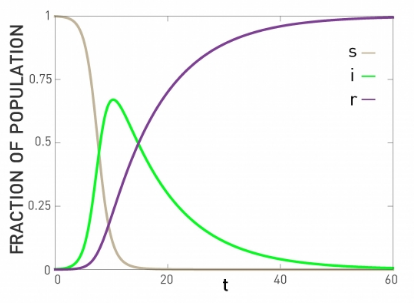
\includegraphics[width=\textwidth]{sir-graphic.png}
%%					\end{subfigure}
%%				\end{figure}
%%			\end{exampleblock}
%%		}
%%		\only<5>{
%%			\begin{information}
%%				{\footnotesize Studies have shown that the airport mobility network provides reliable information for the prediction and control of airborne epidemics like H1N1 \parencite{SorianoPaos2022}.}
%%			\end{information}
%%		}
%%	\end{minipage}
%\end{frame}

\section{The Threshold Model}

\begin{frame}{Modeling Contagion on Graphs: Threshold Model}
	
\onslide<1->{
\begin{itemize}

    \item<1-> Let's consider each vertex as an individual.
    \begin{itemize}
        \item<1-> A vertex is either \textbf{active (infected)} or \textbf{inactive (susceptible)}.
    \end{itemize}
    \item<1-> The individuals change their state based on their neighbors' state.
%    \begin{itemize}
%        \item<2-> A threshold value represents \textbf{how susceptible} an individual is to the contagious agent.
%        \item<2-> Smaller thresholds: early adopters / low immunity;
%        \item<4-> Bigger thresholds: laggards / greater resistance.
%    \end{itemize}
\end{itemize}
}
\onslide<2->{
	\only<2>{
		\begin{figure}
			\centering
			\tikz \graph [spring layout, nodes={draw,circle}] { a[label=above:{\textcolor{red}{1}}] -- {u[fill=red], w, x[fill=red], y, z[fill=red]} };
		\end{figure}
	}
	
	\only<3>{
		\begin{figure}
			\centering
			\tikz \graph [spring layout, nodes={draw,circle}] { a[fill=red, label=above:{\textcolor{red}{1}}] -- {u[fill=red], w, x[fill=red], y, z[fill=red]} };
		\end{figure}
	}
	
	\only<4>{
		\begin{figure}
			\centering
			\tikz \graph [spring layout, nodes={draw,circle}] { a[label=above:{\textcolor{blue}{5}}] -- {u[fill=red], w, x[fill=red], y, z[fill=red]} };
		\end{figure}
	}
}
    
\end{frame}

\begin{frame}{Modeling Contagion on Graphs: Threshold Model}
	In the threshold model, we are given:
	\begin{itemize}
		\item<1-> A \textbf{graph} $G=(V, E)$;
		\item<2-> A \textbf{threshold function} $t:V(G) \rightarrow \mathbb{N}$;
		\item<3-> A set of \textbf{initial infected vertices} -- the \textit{seed set} $S \subseteq V(G)$.
		\item<4-> The diffusion happens in \textbf{discrete time steps}.
		\item<6-> Once a vertex is infected, it \textbf{stays infected} -- we call it a \textbf{$t$-irreversible process}.
	\end{itemize}
	
	\only<1>{
		\begin{figure}
			\centering
			\tikz \graph [spring layout, nodes={draw,circle}, horizontal=a to g] {
				a -- {b, c};
				b -- {c, d, e};
				d -- {[clique] e, f, g}
			};
		\end{figure}
	}
	
	\only<2>{
		\begin{figure}
			\centering
			\tikz \graph [spring layout, nodes={draw,circle}, horizontal=a to g] {
				a[label=below:{\textcolor{red}{2}}] -- {b[label=left:{\textcolor{red}{3}}], c[label=above:{\textcolor{red}{1}}]};
				b -- {c, d, e[label=above:{\textcolor{red}{3}}]};
				d[label=below:{\textcolor{red}{1}}] -- {[clique] e, f[label=above:{\textcolor{red}{2}}], g[label=below:{\textcolor{red}{2}}]}
			};
		\end{figure}
	}
	
	\only<3-4>{
		\begin{figure}
			\centering
			\tikz \graph [spring layout, nodes={draw,circle}, horizontal=a to g] {
				a[fill=red, label=below:{\textcolor{red}{2}}] -- {b[label=left:{\textcolor{red}{3}}], c[label=above:{\textcolor{red}{1}}]};
				b -- {c, d, e[fill=red, label=above:{\textcolor{red}{3}}]};
				d[label=below:{\textcolor{red}{1}}] -- {[clique] e, f[label=above:{\textcolor{red}{2}}], g[label=below:{\textcolor{red}{2}}]};
			};
		\end{figure}
	}
	
	\only<5>{
		\begin{figure}
			\centering
			\tikz \graph [spring layout, nodes={draw,circle}, horizontal=a to g] {
				a[fill=red, label=below:{\textcolor{red}{2}}] -- {b[label=left:{\textcolor{red}{3}}], c[fill=red, label=above:{\textcolor{red}{1}}]};
				b -- {c, d[fill=red, label=below:{\textcolor{red}{1}}], e[fill=red, label=above:{\textcolor{red}{3}}]};
				d -- {[clique] e, f[label=above:{\textcolor{red}{2}}], g[label=below:{\textcolor{red}{2}}]};
			};
		\end{figure}
	}
	
	\only<6>{
		\begin{figure}
			\centering
			\tikz \graph [spring layout, nodes={draw,circle}, horizontal=a to g] {
				a[fill=red, label=below:{\textcolor{red}{2}}] -- {b[fill=red, label=left:{\textcolor{red}{3}}], c[fill=red, label=above:{\textcolor{red}{1}}]};
				
				b -- {c, d[fill=red, label=below:{\textcolor{red}{1}}], e[fill=red, label=above:{\textcolor{red}{3}}]};
				d -- {[clique] e, f[fill=red, label=above:{\textcolor{red}{2}}], g[fill=red, label=below:{\textcolor{red}{2}}]};
			};
		\end{figure}
	}
\end{frame}

\begin{frame}{Problems arising from the Threshold Model}
	Several computational problems arise from the Threshold Model.
	\begin{itemize}
		\item<1-> \textbf{Influence Maximization} (\textsc{IM}) \parencite{kempe}. $\NP$-complete.
		\item<1-> \textbf{Target Set Selection} (\textsc{TSS}) \parencite{DREYER2009}. $\NP$-complete.
		\item<1-> Variations:
		\begin{itemize}
			\item<1-> Directed version;
			\item<1-> Majority version: $t(v) = \lceil \frac{d(v)}{2} \rceil \quad \forall v \in V(G)$;
			\item<1-> \textsc{TSS} with maximum activation time \parencite{Keiler2023, Flocchini2003, Marcilon2018};
			\item<1-> \textsc{TSS} with activation time equal to~1 \parencite{Arajo2023};
		\end{itemize}
%		\begin{itemize}
%			\item<2-> Decision version is  even for bipartite graphs.
%			\item<3-> \NP-complete even for $k$-regular graphs if we require $S$ to infect all vertices of $G$ -- \textbf{Target Set Selection} (\textsc{TSS}) .
%		\end{itemize}
	\end{itemize}
\end{frame}

%\begin{frame}{Problems arising from the Threshold Model}
%	
%	\onslide<1->{
%		Variations of these problems:
%		\begin{itemize}
%			\item Directed version;
%			\item Majority version: $t(v) = \lceil \frac{d(v)}{2} \rceil \quad \forall v \in V(G)$;
%			\item \textsc{TSS} with maximum activation time \parencite{Keiler2023, Flocchini2003, Marcilon2018};
%			\item \textsc{TSS} with activation time equal to~1 \parencite{Arajo2023};
%		\end{itemize}
%	}
%\end{frame}

\begin{frame}{Problems arising from the Threshold Model}
	
	\textbf{Immunization problems}:
	
	\begin{itemize}
		\item<1-> \textbf{Firefighter};
%		\begin{itemize}
%			\item<1-> A fire breaks at some vertex and will spread;
%			\item<2-> The goal is to place firefighters to protect the vertices from the fire.
%			\item<5-> \NP-complete \textbf{even for trees!} (And a bunch of other classes)
%		\end{itemize}
		\item<6-> \textbf{Influence Immunization Bounding} (\textsc{IIB});
		\begin{itemize}
			\item<6-> A generalization of Firefighter? %\textbf{No, but sort of...}
		\end{itemize}
	\end{itemize}
	
	\only<1>{
		\begin{figure}
		\centering
		\begin{tikzpicture}
			\scoped [tree layout]
			\node {\pgfuseimage{fire}}
			child { node {\pgfuseimage{tree}} child { node {\pgfuseimage{tree}}} child { node {\pgfuseimage{tree}}  child { node {\pgfuseimage{tree}}} child { node {\pgfuseimage{tree}}}}  }
			child { node {\pgfuseimage{tree}}  child { node {\pgfuseimage{tree}}} child { node {\pgfuseimage{tree}}} child { node {\pgfuseimage{tree}}} };
		\end{tikzpicture}
		\end{figure}
	}
	
	\only<2>{
		\begin{figure}
			\centering
			\begin{tikzpicture}
				\scoped [tree layout]
				\node {\pgfuseimage{fire}}
				child { node {\pgfuseimage{tree}} child { node {\pgfuseimage{tree}}} child { node {\pgfuseimage{tree}}  child { node {\pgfuseimage{tree}}} child { node {\pgfuseimage{tree}}}}  }
				child { node {\pgfuseimage{fighter}}  child { node {\pgfuseimage{tree}}} child { node {\pgfuseimage{tree}}} child { node {\pgfuseimage{tree}}} };
			\end{tikzpicture}
		\end{figure}
	}
	
	\only<3>{
		\begin{figure}
			\centering
			\begin{tikzpicture}
				\scoped [tree layout]
				\node {\pgfuseimage{fire}}
				child { node {\pgfuseimage{fire}} child { node {\pgfuseimage{tree}}} child { node {\pgfuseimage{tree}}  child { node {\pgfuseimage{tree}}} child { node {\pgfuseimage{tree}}}}  }
				child { node {\pgfuseimage{fighter}}  child { node {\pgfuseimage{tree}}} child { node {\pgfuseimage{tree}}} child { node {\pgfuseimage{tree}}} };
			\end{tikzpicture}
		\end{figure}
	}
	
	\only<4>{
		\begin{figure}
			\centering
			\begin{tikzpicture}
				\scoped [tree layout]
				\node {\pgfuseimage{fire}}
				child { node {\pgfuseimage{fire}} child { node {\pgfuseimage{tree}}} child { node {\pgfuseimage{fighter}}  child { node {\pgfuseimage{tree}}} child { node {\pgfuseimage{tree}}}}  }
				child { node {\pgfuseimage{fighter}}  child { node {\pgfuseimage{tree}}} child { node {\pgfuseimage{tree}}} child { node {\pgfuseimage{tree}}} };
			\end{tikzpicture}
		\end{figure}
	}
	
	\only<5->{
		\begin{figure}
			\centering
			\begin{tikzpicture}
				\scoped [tree layout]
				\node {\pgfuseimage{fire}}
				child { node {\pgfuseimage{fire}} child { node {\pgfuseimage{fire}}} child { node {\pgfuseimage{fighter}}  child { node {\pgfuseimage{tree}}} child { node {\pgfuseimage{tree}}}}  }
				child { node {\pgfuseimage{fighter}}  child { node {\pgfuseimage{tree}}} child { node {\pgfuseimage{tree}}} child { node {\pgfuseimage{tree}}} };
			\end{tikzpicture}
		\end{figure}
	}
	
\end{frame}

\section{Influence Immunization Bounding}

\begin{frame}{Influence Immunization Bounding}
	First, we need to define what it means to \textbf{immunize a vertex}.
	
	\begin{itemize}
		\item<1-> Option 1: raise the vertex threshold above its degree;
		\item<1-> \textcolor{red}{\textbf{Option 2: make the vertex invisible -- remove it.}}
	\end{itemize}
	
%	\only<1>{
%		\begin{figure}
%			\centering
%			\tikz \graph [spring layout, nodes={draw,circle}] { a[label=above:{\textcolor{red}{$+\infty$}}, draw=blue, line width=1mm] -- {u[fill=red], w[label=left:{\textcolor{red}{1}}], x[fill=red], y[label=right:{\textcolor{red}{1}}], z[fill=red]} };
%		\end{figure}
%	}
%	
%	\only<2>{
%		\begin{minipage}[c]{0.5\textwidth}
%			\begin{figure}
%				\centering
%				\tikz \graph [spring layout, nodes={draw,circle}] { a[label=above:{\textcolor{red}{3}}] -- {u[fill=red], w[label=left:{\textcolor{red}{1}}], x[label=left:{\textcolor{red}{$+\infty$}}, draw=blue, line width=1mm, fill=red], y[label=right:{\textcolor{red}{1}}], z[fill=red]} };
%			\end{figure}
%		\end{minipage}\begin{minipage}[c]{0.5\textwidth}
%			\begin{remark}[Option 1]
%				Infected vertices can also be immunized. In this option, the immunized infected vertices still \textbf{can infect others}.
%			\end{remark}
%		\end{minipage}
%	}
%	
%	\only<3>{
%		\begin{minipage}[c]{0.5\textwidth}
%			\begin{figure}
%				\centering
%				\tikz \graph [spring layout, nodes={draw,circle}] { a[label=above:{\textcolor{red}{3}}, fill=red] -- {u[fill=red], w[label=left:{\textcolor{red}{1}}], x[label=left:{\textcolor{red}{$+\infty$}}, draw=blue, line width=1mm, fill=red], y[label=right:{\textcolor{red}{1}}], z[fill=red]} };
%			\end{figure}
%		\end{minipage}\begin{minipage}[c]{0.5\textwidth}
%			\begin{remark}[Option 1]
%				Infected vertices can also be immunized. In this option, the immunized infected vertices still \textbf{can infect others}.
%			\end{remark}
%		\end{minipage}
%	}
	
	
		\begin{minipage}[c]{0.5\textwidth}
			\begin{figure}
				\centering
				\tikz \graph [spring layout, nodes={draw,circle}] {
					a --[dashed] x[label=left:{\textcolor{red}{$+\infty$}}, line width=1mm, fill=red, dashed, draw=blue];
					
					a[label=above:{\textcolor{red}{3}}] -- {u[fill=red], w[label=left:{\textcolor{red}{1}}], y[label=right:{\textcolor{red}{1}}], z[fill=red]};							
				};
				
			\end{figure}
		\end{minipage}\begin{minipage}[c]{0.5\textwidth}
			\onslide<2->{\begin{remark}[Option 2]
				In this option, immunized vertices do not infect nor get infected.
			\end{remark}}
		\end{minipage}
	
\end{frame}

\begin{frame}{Influence Immunization Bounding}
	
	\begin{minipage}[t]{0.6\textwidth}
		\onslide<1->{
			Given:
			\begin{itemize}
				\item<1-> A graph $G=(V, E)$ with thresholds $t:V(G) \rightarrow \mathbb{N}$;
				\item<2-> A seed set $S \subseteq V(G)$;
				\item<5-> Naturals $k$ and $l$. \only<6->{\textbf{Let $k=3$ and $l=2$.}}
			\end{itemize}
		}
		
		\onslide<6->{
			We want to find a immunizing set $Y \subseteq V(G)$ such that:
			\begin{itemize}
				\item<6-> $|Y| \leq l$; and
				\item<7-> By immunizing $Y$ at time $\tau=0$, the \textbf{infection gets restricted to at most $k$ vertices}.
			\end{itemize}
		}
		
		\only<2-4>{
			\begin{remark}
				Notice that $S = \{a, e, h\}$ is a \textit{target set} for this graph.
			\end{remark}
		}
		\only<7->{
			\begin{remark}
				Notice that we must have $k \geq |S|$.
			\end{remark}
		}
	\end{minipage}\begin{minipage}[t]{0.4\textwidth}
		\only<1>{
			\begin{figure}
				\centering
				\tikz \graph [spring layout, nodes={draw,circle}] {
					{[clique] a[label=above:{\textcolor{red}{1}}], b[label=above:{\textcolor{red}{2}}], c[label=left:{\textcolor{red}{1}}], d[label=right:{\textcolor{red}{3}}]};
					{[clique] c, d, e[label=left:{\textcolor{red}{1}}], f[label=right:{\textcolor{red}{2}}]};
					{[clique] e, f, g[label=above:{\textcolor{red}{2}}]};
					g -- h[label=left:{\textcolor{red}{1}}];
				};
				
			\end{figure}
		}
		\only<2>{
			\begin{figure}
				\centering
				\tikz \graph [spring layout, nodes={draw,circle}] {
					{[clique] a[label=above:{\textcolor{red}{1}}, fill=red], b[label=above:{\textcolor{red}{2}}], c[label=left:{\textcolor{red}{1}}], d[label=right:{\textcolor{red}{3}}]};
					{[clique] c, d, e[fill=red, label=left:{\textcolor{red}{1}}], f[label=right:{\textcolor{red}{2}}]};
					{[clique] e, f, g[label=above:{\textcolor{red}{2}}]};
					g -- h[fill=red, label=left:{\textcolor{red}{1}}];
				};
				
			\end{figure}
		}
		\only<3>{
			\begin{figure}
				\centering
				\tikz \graph [spring layout, nodes={draw,circle}] {
					{[clique] a[label=above:{\textcolor{red}{1}}, fill=red], b[label=above:{\textcolor{red}{2}}], c[fill=red, label=left:{\textcolor{red}{1}}], d[label=right:{\textcolor{red}{3}}]};
					{[clique] c, d, e[fill=red, label=left:{\textcolor{red}{1}}], f[label=right:{\textcolor{red}{2}}]};
					{[clique] e, f, g[fill=red, label=above:{\textcolor{red}{2}}]};
					g -- h[fill=red, label=left:{\textcolor{red}{1}}];
				};
				
			\end{figure}
		}
		\only<4>{
			\begin{figure}
				\centering
				\tikz \graph [spring layout, nodes={draw,circle}] {
					{[clique] a[label=above:{\textcolor{red}{1}}, fill=red], b[label=above:{\textcolor{red}{2}}, fill=red], c[fill=red, label=left:{\textcolor{red}{1}}], d[label=right:{\textcolor{red}{3}}, fill=red]};
					{[clique] c, d, e[fill=red, label=left:{\textcolor{red}{1}}], f[label=right:{\textcolor{red}{2}}, fill=red]};
					{[clique] e, f, g[fill=red, label=above:{\textcolor{red}{2}}]};
					g -- h[fill=red, label=left:{\textcolor{red}{1}}];
				};
				
			\end{figure}
		}
		\only<5>{
			\begin{figure}
				\centering
				\tikz \graph [spring layout, nodes={draw,circle}] {
					{[clique] a[label=above:{\textcolor{red}{1}}, fill=red], b[label=above:{\textcolor{red}{2}}], c[label=left:{\textcolor{red}{1}}], d[label=right:{\textcolor{red}{3}}]};
					{[clique] c, d, e[fill=red, label=left:{\textcolor{red}{1}}], f[label=right:{\textcolor{red}{2}}]};
					{[clique] e, f, g[label=above:{\textcolor{red}{2}}]};
					g -- h[fill=red, label=left:{\textcolor{red}{1}}];
				};
				
			\end{figure}
		}
		\only<6->{
			\begin{figure}
				\centering
				\tikz \graph [spring layout, nodes={draw,circle}] {
					{[clique] a[label=above:{\textcolor{red}{1}}, fill=red], b[label=above:{\textcolor{red}{2}}], c[label=left:{\textcolor{red}{1}}, draw=blue, line width=1mm], d[label=right:{\textcolor{red}{3}}]};
					{[clique] c, d, e[fill=red, label=left:{\textcolor{red}{1}}], f[label=right:{\textcolor{red}{2}}]};
					{[clique] e, f, g[label=above:{\textcolor{red}{2}}]};
					g -- h[fill=red, label=left:{\textcolor{red}{1}}, draw=blue, line width=1mm];
				};
				
			\end{figure}
		}
	\end{minipage}
	
\end{frame}

\section{Parameterized Complexity}

\begin{frame}
	\textit{But before we proceed...}
	
	A little of \textbf{Parameterized Complexity}.
\end{frame}

%\begin{frame}{Parameterized Complexity}
%	We can define a (classical) decision problem as follows:
%	\begin{itemize}
%		\item<1-> Let $\Sigma$ be a finite alphabet, and $Q \subseteq \Sigma^*$.
%	\end{itemize}
%	\onslide<1->{
%		\noindent\makebox[\textwidth][c]{%
%			\begin{minipage}{0.5\textwidth}
%				\begin{framed}
%					\textit{Input}: $x \in \Sigma^*$.\\
%					\textit{Question}: Decide whether $x \in Q$.
%				\end{framed}
%		\end{minipage}}
%	}
%	\onslide<2->{
%		\begin{minipage}{0.45\textwidth}
%			\begin{definition}
%				A \textbf{parameter} is a function $\kappa:\Sigma^* \rightarrow \mathbb{N}$ that takes the input of a problem to the naturals.
%			\end{definition}
%		\end{minipage}\hfill\begin{minipage}{0.45\textwidth}
%		\begin{example}
%			A parameter for \textsc{SAT} can be $\kappa(\varphi) = \text{``Number of variables of $\varphi$''}$, where $\varphi$ is a CNF formula.
%		\end{example}
%		\end{minipage}
%	}
%\end{frame}

\begin{frame}{Parameterized Complexity}
	%Let's define a \textbf{parameterized problem}.
	
	\begin{definition}
		A \textit{parameterized problem} is a pair $(P, \kappa)$, such that $P$ is a decision problem and $\kappa$ is a parameter for $P$.
	\end{definition}
	
	\onslide<1->{
		\noindent\makebox[\textwidth][c]{%
			\begin{minipage}{0.75\textwidth}
				\begin{framed}
					p-\textsc{Independent-Set}\\
					\textit{Input}: A graph $G$ and $k \in \mathbb{N}$.\\
					\textit{Question}: Decide whether $G$ has an independent set of cardinality $k$.\\
					\textbf{Parameter}: $k$.
				\end{framed}
		\end{minipage}}
	}
	
	\textcolor{red}{\textbf{Parameters of the problem matter for its tractability.}}
\end{frame}

%\begin{frame}{Parameterized Complexity}
%	But what is the motivation behind this?
%	\begin{itemize}
%		\item<1-> \NP-hard problems cannot have \textbf{all instances} solved in polynomial time, unless $\P = \NP$.
%		\item<2-> But in practice, \textbf{only a subset} of them is relevant.
%		\begin{itemize}
%			\item<2-> VLSI design: the number of circuit layers is \textcolor{red}{usually $\leq 10$};
%			\item<2-> Computational biology: real instances of DNA chain reconstruction have special properties, e.g., \textcolor{red}{treewidth $\leq 11$};
%			\item<2-> Robotics: the number of degrees of freedom in motion planning problems is \textcolor{red}{usually $\leq 10$}.
%		\end{itemize}
%		\item<3-> This means that \textbf{parameters of the problem matter for its tractability}.
%	\end{itemize}
%\end{frame}

\begin{frame}{Parameterized Complexity}
	Let $x \in \Sigma^*$ be an instance of a parameterized problem $(P, \kappa)$.
	\onslide<1->{
		\begin{definition}[$\XP$]
			$(P, \kappa)$ is \textbf{slicewise polynomial} if it admits an algorithm which running time is $$O(|x|^{\kappa(x)})$$
		\end{definition}
		\only<1>{
			\begin{itemize}
				\item \textsc{Clique} is in $\XP$ parameterized by $k$: enumerate all subsets of $k$ vertices and check if they form a clique.
			\end{itemize}
		}
	}

	\onslide<2->{
		\begin{definition}[$\FPT$]
			$(P, \kappa)$ is \textbf{fixed-parameter tractable} if it admits an algorithm which running time is $$O(f(\kappa(x))\cdot poly(|x|))$$
		\end{definition}
		\only<2>{
			\begin{itemize}
				\item \textsc{Vertex Cover} is in $\FPT$ parameterized by $k$.
			\end{itemize}
		}
	}
\end{frame}

\begin{frame}
	\begin{itemize}
		\item<1-> The class $\FPT$ is the parameterized analogous to the class $\P$;
		\item<1-> The class para-$\NP$ is the parameterized analogous to the class $\NP$;
		\item<2-> $k$-\textsc{Clique} is the parameterized analogous to \textsc{3-Sat};
		\begin{itemize}
			\item<2-> No one has managed to find a $\FPT$ algorithm;
			\item<2-> \textbf{Hypothesis: $k$-\textsc{Clique} is not in $\FPT$.}
		\end{itemize}
		\item<3-> The $\W[t]$-hardness is the parameterized analogous of $\NP$-hardness.
		\begin{itemize}
			\item<3-> $k$-\textsc{Clique} is $\W[1]$-hard;
			\item<3-> \textsc{Hitting Set} and \textsc{Dominating Set} are $\W[2]$-hard;
			\item<3-> We can show other problems are $\W[t]$-hard by using $\FPT$-reductions.
		\end{itemize}
	\end{itemize}
\end{frame}

\section{Influence Immunization Bounding (cont.)}

\begin{frame}{Influence Immunization Bounding (cont.)}
	\fullcite{Cordasco2023}
	%Influence Immunization Bounding was introduced by \parencite{Cordasco2023}.
	%\begin{itemize}
	%	\item<1-> $\W[1]$-hard parameterized by $k$ or by $l$ even if $t(v)=1 \quad \forall v \in V(G)$;
	%	\item<1-> $\W[1]$-hard parameterized by the neighborhood diversity $nd(G)$;
	%	\item<1-> $\W[1]$-hard parameterized by the treewidth $tw(G)$;
	%	\item<2-> $\W[2]$-hard parameterized by $|S|+l$ even on bipartite graphs;
	%	\item<2-> $\W[2]$-hard parameterized by $\Delta(G) + l$ even if $t(v) \leq 2 \quad \forall v \in V(G)$.
	%	\item<3-> $\FPT$ parameterized by $k + l$;
	%	\item<3-> $\FPT$ parameterized by $k + |S|$;
	%	\item<3-> $\FPT$ parameterized by $min(\Delta(G), k)+tw(G)+l$;
	%	\item<3-> $\FPT$ parameterized by $k + nd(G)$;
	%	\item<3-> $\FPT$ parameterized by $l + nd(G)$.
	%\end{itemize}
	\begin{center}
		\begin{tabular}{ c | c  c }
			%\hline
			\textbf{Parameter} & \textbf{Hardness} & \\
			%\hline
			$k$ & $\W[1]$-hard & $t(v)=1 \quad \forall v$ \\
			$l$ & $\W[1]$-hard & $t(v)=1 \quad \forall v$ \\
			$k+l$ & $\FPT$ &  \\
			$|S| + l$ & $\W[2]$-hard & Bipartite graphs \\
			$k+|S|$ & $\FPT$ & \\
			$\Delta(G) + l$ & $\W[2]$-hard & $t(v) \leq 2 \quad \forall v$ \\
			$tw(G)$ & $\W[1]$-hard & \\
			$nd(G)$ & $\W[1]$-hard & \\
			$k+nd(G)$ & $\FPT$ & \\
			$l+nd(G)$ & $\FPT$ & \\
			$\min(\Delta(G), k)+tw(G)+l$ & $\FPT$ & \\
			%\hline
		\end{tabular}
	\end{center}
	
	
	
\end{frame}

\begin{frame}{Influence Immunization Bounding (cont.)}
	Let $G=(V,E)$ be a graph with thresholds $t:V(G) \rightarrow \mathbb{N}$ and seed set $S \subseteq V(G)$.
	
	\begin{definition}
		Let $Y \subseteq V(G)$. If, by immunizing the vertices of $Y$, the infection in $(G, t)$ is restricted to \textbf{at most} $k$ vertices, we say that $Y$ is a \textbf{$k$-restricting set}.
	\end{definition}
	
	\begin{definition}
		The \textbf{$k$-restricting number of $(G, t)$}, denoted by $$\mathfrak{R}(G, t, k)$$, is size of a \textbf{mimimum $k$-restricting set} of $(G, t)$.
	\end{definition}
\end{frame}

\begin{frame}{Influence Immunization Bounding (cont.)}
	
	\begin{minipage}[t]{0.6\textwidth}
		\onslide<1->{
			Consider the graph on the right.
			\begin{example}
				$Y = \{c, h\}$ is a $3$-restricting set of $(G, t)$.
				
				$\mathfrak{R}(G, t, k=3) = 2$.
			\end{example}
		}
		\onslide<2->{
			\begin{Definition}
				If $k = |S|$, then we say that $\mathfrak{R}(G, t, k=|S|)$ is the \textbf{total restricting number of $(G, t)$}, and denote it by $\mathfrak{R}_T(G, t)$.
			\end{Definition}
			
			\begin{example}
				$\mathfrak{R}_T(G, t) = \mathfrak{R}(G, t, k=3)=2$.
			\end{example}
		}
		
		\onslide<3->{
			\begin{remark}
				For any suitable $k$, we have that $$\mathfrak{R}(G, t, k) \leq \mathfrak{R}_T(G, t)$$
			\end{remark}
		}
	\end{minipage}\begin{minipage}[t]{0.4\textwidth}
		\only<1->{
			\begin{figure}
				\centering
				\tikz \graph [spring layout, nodes={draw,circle}] {
					{[clique] a[label=above:{\textcolor{red}{1}}, fill=red], b[label=above:{\textcolor{red}{2}}], c[label=left:{\textcolor{red}{1}}, draw=blue, line width=1mm], d[label=right:{\textcolor{red}{3}}]};
					{[clique] c, d, e[fill=red, label=left:{\textcolor{red}{1}}], f[label=right:{\textcolor{red}{2}}]};
					{[clique] e, f, g[label=above:{\textcolor{red}{2}}]};
					g -- h[fill=red, label=left:{\textcolor{red}{1}}, draw=blue, line width=1mm];
				};
				
			\end{figure}
		}
	\end{minipage}
	
\end{frame}

%\begin{frame}{Influence Immunization Bounding (cont.)}
%	We can also define a \textbf{restricted version} of \textsc{IIB}, which we call \textsc{r-IIB}.
%	
%	\onslide<1->{
%		\noindent\makebox[\textwidth][c]{%
%			\begin{minipage}{0.70\textwidth}
%				\begin{framed}
%					\textbf{Restricted Influence Immunization Bounding} (\textsc{r-IIB})\\
%					\textit{Input}: A graph $G=(V, E)$ with thresholds $t:V(G) \rightarrow \mathbb{N}$, seed set $S \subseteq V(G)$, and $k, l \in \mathbb{N}$.\\
%					\textit{Question}: Decide whether there exists $Y \subseteq \textcolor{red}{V(G) \setminus S}$ such that $|Y| \leq l$ and $Y$ is a $k$-immunizing set of $G$.
%				\end{framed}
%		\end{minipage}}
%	}
%	
%	\begin{itemize}
%		\item \textsc{r-IIB} is also $\W[1]$-hard when parameterized by $k$ or by $l$.
%	\end{itemize}
%\end{frame}
%
%\begin{frame}{Influence Immunization Bounding (cont.)}
%	
%	\begin{minipage}[t]{0.6\textwidth}
%		\only<1-2>{
%			Consider the graph on the right.
%			
%			\begin{definition}
%				$Y \subseteq V(G)$ is a \textbf{restricted $k$-immunizing set} of $(G, t)$ if $Y$ is a $k$-immunizing set of $(G, t)$ and $Y \cap S = \emptyset$.
%			\end{definition}
%			
%			\begin{itemize}
%				\item<1-> \textcolor{red}{\textbf{$Y = \{c, h\}$ is \underline{not} a restricted $k$-immunizing set of $(G, t)$.}}.
%				\item<2-> \textcolor{blue}{\textbf{$Y = \{c, g\}$ \underline{is} a restricted $k$-immunizing set of $(G, t)$.}}
%			\end{itemize}
%		}
%		
%		\only<3->{
%			\begin{definition}
%				The \textbf{restricted $k$-immunization number of $(G, t)$}, denoted by $$\text{Im}_r(G, t, k)$$, is the size of a \textbf{mimimum restricted $k$-immunizing set} of $(G, t)$.
%			\end{definition}
%			
%			\begin{itemize}
%				\item The \textbf{restricted inhibition number} $\text{In}_r(G, t)$ is analogous.
%				\item \textbf{But why study the restricted version?}
%			\end{itemize}
%			
%		}
%			
%	\end{minipage}\begin{minipage}[t]{0.4\textwidth}
%		\only<1>{
%			\begin{figure}
%				\centering
%				\tikz \graph [spring layout, nodes={draw,circle}] {
%					{[clique] a[label=above:{\textcolor{red}{1}}, fill=red], b[label=above:{\textcolor{red}{2}}], c[label=left:{\textcolor{red}{1}}, draw=blue, line width=1mm], d[label=right:{\textcolor{red}{3}}]};
%					{[clique] c, d, e[fill=red, label=left:{\textcolor{red}{1}}], f[label=right:{\textcolor{red}{2}}]};
%					{[clique] e, f, g[label=above:{\textcolor{red}{2}}]};
%					g -- h[fill=red, label=left:{\textcolor{red}{1}}, draw=blue, line width=1mm];
%				};
%				
%			\end{figure}
%		}
%		
%		\only<2->{
%			\begin{figure}
%				\centering
%				\tikz \graph [spring layout, nodes={draw,circle}] {
%					{[clique] a[label=above:{\textcolor{red}{1}}, fill=red], b[label=above:{\textcolor{red}{2}}], c[label=left:{\textcolor{red}{1}}, draw=blue, line width=1mm], d[label=right:{\textcolor{red}{3}}]};
%					{[clique] c, d, e[fill=red, label=left:{\textcolor{red}{1}}], f[label=right:{\textcolor{red}{2}}]};
%					{[clique] e, f, g[label=above:{\textcolor{red}{2}}, draw=blue, line width=1mm]};
%					g -- h[fill=red, label=left:{\textcolor{red}{1}}];
%				};
%				
%			\end{figure}
%		}
%		
%	\end{minipage}
%	
%\end{frame}
%
%\begin{frame}{Influence Immunization Bounding (cont.)}
%	The restricted version gives an upper bound for the original problem.
%	
%	\begin{remark}
%		For any suitable $k$, we have that $$\text{Im}(G, t, k) \leq \text{Im}_r(G, t, k)$$
%	\end{remark}
%	
%	\begin{itemize}
%		\item<1-> A restricted $k$-immunizing set for $(G, t)$ is also a (unrestricted) $k$-immunizing set for $(G, t)$.
%	\end{itemize}
%\end{frame}

\section{Related Work}

\begin{frame}{Related Work}
	\begin{itemize}
		\item \fullcite{Fomin_Cutting}
		\item \fullcite{Hayrapetyan2005}
		\item \fullcite{Mehta2022}
	\end{itemize}
\end{frame}

\begin{frame}{Related Work}
	\begin{itemize}
		\item Firefighter is very conceptually related \parencite{Anshelevich2010};
		\item Game theoretical approach \parencite{Aspnes2006,Chen2010,Moscibroda2006,Meier2014};
		\item Spectral graph theory \parencite{Ahmad2020, Chen2016, Chakrabarti2008, Tariq2017}.
	\end{itemize}
	
\end{frame}

\section{Our Results}

%\begin{frame}
%	\sectionpage
%\end{frame}

\begin{frame}{}
	\textbf{\huge Our Results}
\end{frame}

\part{Paths and Complete Graphs with $t(v) = c$}

%\begin{frame}
%	\partpage
%\end{frame}

\subsection{A bound for paths with $t(v)=2$}

\begin{frame}{Paths with $t(v)=2$}
	
	\begin{definition}
		Let $G = (V, E)$ be a graph and $S \subseteq V(G)$ a seed set of $G$. Then $P = v_1 v_2 \dots v_k$ is a \textbf{$S$-alternating path} of $G$ if $P$ is a path of $G$ with \textit{at least~3 vertices} and the vertices of $P$ alternate with respect to their membership in $S$.
	\end{definition}
	
	\begin{figure}[h]
		\centering
		\begin{subfigure}{0.45\textwidth}
			\centering
			\begin{tikzpicture}[scale=0.8, every node/.style={circle, draw, inner sep=0pt, minimum size=6pt}]
				\foreach \x in {0,...,4}
				{
					\ifodd\x
					\node (\x) at (\x,0) [fill=white] {};
					\else
					\node (\x) at (\x,0) [fill=black] {};
					\fi
				}
				\draw (0) -- (1) -- (2) -- (3) -- (4);
			\end{tikzpicture}
		\end{subfigure}
		\hfill
		\begin{subfigure}{0.45\textwidth}
			\centering
			\begin{tikzpicture}[scale=0.8, every node/.style={circle, draw, inner sep=0pt, minimum size=6pt}]
				\foreach \x in {0,...,4}
				{
					\ifodd\x
					\node (\x) at (\x,0) [fill=black] {};
					\else
					\node (\x) at (\x,0) [fill=white] {};
					\fi
				}
				\draw (0) -- (1) -- (2) -- (3) -- (4);
			\end{tikzpicture}
		\end{subfigure}
	\end{figure}
	
\end{frame}

\begin{frame}{Paths with $t(v)=2$}
	\begin{itemize}
		\item \textbf{Main observation:} for each $S$-alternating path of length~4, \textbf{we need only one vertex to inhibit} the infection.
	\end{itemize}
	
	\begin{figure}[h]
		\centering
		\begin{subfigure}{0.45\textwidth}
			\centering
			\begin{tikzpicture}[scale=0.8, every node/.style={circle, draw, inner sep=0pt, minimum size=6pt}]
				\foreach \x in {0,...,3}
				{
					\ifodd\x
					\node (\x) at (\x,0) [fill=white] {};
					\else
					\node (\x) at (\x,0) [fill=black] {};
					\fi
				}
				\draw (0) -- (1) -- (2) -- (3);
				
				\node[draw=blue, rectangle, inner sep=5pt, fit=(2)] {};
			\end{tikzpicture}
		\end{subfigure}
		\hfill
		\begin{subfigure}{0.45\textwidth}
			\centering
			\begin{tikzpicture}[scale=0.8, every node/.style={circle, draw, inner sep=0pt, minimum size=6pt}]
				\foreach \x in {0,...,3}
				{
					\ifodd\x
					\node (\x) at (\x,0) [fill=black] {};
					\else
					\node (\x) at (\x,0) [fill=white] {};
					\fi
				}
				\draw (0) -- (1) -- (2) -- (3);
				
				\node[draw=blue, rectangle, inner sep=5pt, fit=(1)] {};
			\end{tikzpicture}
		\end{subfigure}
		\caption{When the $S$-alternating paths has length~4, we can inhibit the infection by immunizing only one vertex.}
	\end{figure}
	
	\begin{figure}[h]
		\centering
		\begin{subfigure}{0.45\textwidth}
			\centering
			\begin{tikzpicture}[scale=0.8, every node/.style={circle, draw, inner sep=0pt, minimum size=6pt}]
				\foreach \x in {0,...,2}
				{
					\ifodd\x
					\node (\x) at (\x,0) [fill=white] {};
					\else
					\node (\x) at (\x,0) [fill=black] {};
					\fi
				}
				\draw (0) -- (1) -- (2);
				
				\node[draw=blue, rectangle, inner sep=5pt, fit=(2)] {};
			\end{tikzpicture}
			\caption{The infection stops by immunizing any vertex. The immunized vertex is shown in blue.}
		\end{subfigure}
		\hfill
		\begin{subfigure}{0.45\textwidth}
			\centering
			\begin{tikzpicture}[scale=0.8, every node/.style={circle, draw, inner sep=0pt, minimum size=6pt}]
				\foreach \x in {0,...,2}
				{
					\ifodd\x
					\node (\x) at (\x,0) [fill=black] {};
					\else
					\node (\x) at (\x,0) [fill=white] {};
					\fi
				}
				\draw (0) -- (1) -- (2);
			\end{tikzpicture}
			\caption{When the $S$-alternating path has length~3 and starts with a uninfected vertex, the infection does not spread.}
			\label{subfig:3-alt-path-unin}
		\end{subfigure}
	\end{figure}

\end{frame}

\begin{frame}{Paths with $t(v)=2$}
	\begin{itemize}
		\item We can split the path into $S$-alternating paths of length~4.
	\end{itemize}
	
	\begin{figure}[h]
		\centering
		\begin{tikzpicture}[scale=0.8, every node/.style={circle, draw, inner sep=0pt, minimum size=6pt}]
			\foreach \x in {0,...,13}
			{
				\ifodd\x
				\node (\x) at (\x,0) [fill=black] {};
				\else
				\node (\x) at (\x,0) [fill=white] {};
				\fi
			}
			\node[draw=none, inner sep=5pt] (-2) at (-2, 0) {$\dots$};
			\node[draw=none, inner sep=5pt] (15) at (15, 0) {$\dots$};
			\node[draw] (-1) at (-1, 0) {};
			\node[draw, fill=black] (14) at (14, 0) {};
			
			\draw (-2) -- (-1) -- (0) -- (1) -- (2) -- (3) -- (4) -- (5) -- (6) -- (7) -- (8) -- (9) -- (10) -- (11) -- (12) -- (13) -- (14) -- (15);
			
			\node[draw=red, rectangle, fit=(1) (2) (3) (4), inner sep=5pt] {};
			\node[draw=red, rectangle, fit=(5) (6) (7) (8), inner sep=5pt] {};
			\node[draw=red, rectangle, fit=(9) (10) (11) (12), inner sep=5pt] {};
			\node[draw, rectangle, fit=(0) (1) (2) (3) (4) (5) (6) (7) (8) (9) (10) (11) (12) (13), inner sep=10pt] {};
			
		\end{tikzpicture}
		\caption{Splitting a bigger $S$-alternating path into pieces of length~4 starting with infected vertices.}
		\label{fig:split-paths}
	\end{figure}
	
	\begin{proposition}
		Let $G = P_n$ with $t(v)=2$ for all $v \in V(G)$. Then, for any $k \in \mathbb{N}$, \[
			\text{Im}(G, t, k) \leq \text{In}(G, t) \leq \lceil \frac{n}{4} \rceil
		\]
	\end{proposition}
\end{frame}

\subsection{Exact value for paths with $t(v)=2$}

%\begin{frame}{Exact value for paths with $t(v)=2$}
%	\begin{definition}
%		Let $G=(V, E)$ be a graph and $S \subseteq V(G)$ a seed set of $G$. Then:
%		\begin{itemize}
%			\item $P=v_1v_2v_3$ is a $\bullet\circ\bullet$-path if $P$ is a \textbf{maximal $S$-alternating path} of length exactly~3 such that $v_1, v_3 \in S$.
%			\item $P=v_1v_2v_3v_4$ is a $\bullet\circ\bullet\circ$-path if $P$ is a $S$-alternating path of length~4 such that $v_1, v_3 \in S$.
%		\end{itemize}
%	\end{definition}
%\end{frame}

\subsection{Complete graphs with $t(v)=c$}

\begin{frame}{Complete graphs with $t(v)=c$}
	\begin{proposition}
		\label{prop:complete-fixed}
		Let $G \cong K_n$ be a complete graph on $n$ vertices with thresholds $t(v) = c$ for all $v \in V(G)$, $S \subseteq V(G)$ a seed set of $G$, and $k \in \mathbb{N}$. Then:
		
		\[
		\text{Im}(G, t, k) =
		\begin{cases}
			\min\{|S|-c+1, n-k\}, & \text{if } |S| \geq c\\
			0, & \text{otherwise.}  
		\end{cases}
		\]
	\end{proposition}
	\begin{figure}[h]
		\centering
		\begin{subfigure}{0.45\textwidth}
			\centering
			\resizebox{!}{.33\textheight}{\begin{tikzpicture}[scale=0.8, every node/.style={circle, draw}]
				
				\node[circle, draw, text=red] (A) {2};
				\node[circle, draw, above right=of A, text=red] (B) {2};
				\node[circle, draw, below right=of B,text=red] (C) {2};
				\node[circle, draw, below=of A, text=red] (D) {2};
				\node[circle, draw, below=of C, fill=red, text=red] (E) {E};
				\node[circle, draw, below right=of D, text=red] (F) {2};
				
				
				% Draw edges between all pairs of nodes
				\draw (A) -- (B);
				\draw (A) -- (C);
				\draw (A) -- (D);
				\draw (A) -- (E);
				\draw (B) -- (C);
				\draw (B) -- (D);
				\draw (B) -- (E);
				\draw (C) -- (D);
				\draw (C) -- (E);
				\draw (D) -- (E);
				\draw (F) -- (E);
				\draw (F) -- (D);
				\draw (F) -- (C);
				\draw (F) -- (B);
				\draw (F) -- (A);
				
			\end{tikzpicture}}
			%\caption{When $|S| < c$, no vertex will ever be infected.}
			%\label{subfig:s_menor_c}
		\end{subfigure}
		\hfill
		\begin{subfigure}{0.45\textwidth}
			\centering
			\resizebox{!}{.33\textheight}{\begin{tikzpicture}[scale=0.8, every node/.style={circle, draw}]
				
				\node[circle, draw, fill=red, text=red] (A) {3};
				\node[circle, draw, above right=of A, text=red, text=red] (B) {3};
				\node[circle, draw, below right=of B, fill=red, text=red] (C) {3};
				\node[circle, draw, below=of A, fill=red, text=red] (D) {3};
				\node[circle, draw, below=of C, fill=red, text=red] (E) {E};
				\node[circle, draw, below right=of D, text=red] (F) {3};
				
				
				% Draw edges between all pairs of nodes
				\draw (A) -- (B);
				\draw (A) -- (C);
				\draw (A) -- (D);
				\draw (A) -- (E);
				\draw (B) -- (C);
				\draw (B) -- (D);
				\draw (B) -- (E);
				\draw (C) -- (D);
				\draw (C) -- (E);
				\draw (D) -- (E);
				\draw (F) -- (E);
				\draw (F) -- (D);
				\draw (F) -- (C);
				\draw (F) -- (B);
				\draw (F) -- (A);
				
				\node[draw=blue, rectangle, fit=(C), inner sep=4pt] {};
				\node[draw=blue, rectangle, fit=(E), inner sep=4pt] {};
				
				\node[draw=green, rectangle, fit=(B), inner sep=4pt] {};
				\node[draw=green, rectangle, fit=(F), inner sep=4pt] {};
				
			\end{tikzpicture}}
			%\caption{Suppose $k = 4$. Then, we have two options: we either immunize $|S| - c + 1 = 2$ infected vertices (blue) or $n - k = 2$ uninfected vertices (green).}
			%\label{subfig:s_maior_c}
		\end{subfigure}
	\end{figure}
\end{frame}

%\part{Polynomial Algorithm for the $k$-Immunization Number in Trees}
%
%\begin{frame}
%	\partpage
%\end{frame}
%
%\begin{frame}{Polynomial Algorithm for Trees}
%	\begin{itemize}
%		\item Para dois naturais $x$ e $y$, defina $$\mathfrak{P}_x(y) = \{(a_1, \dots, a_x) \in \mathbb{N}^x \mid a_1 + \dots + a_x = y\}$$
%	\end{itemize}
%\end{frame}

%\part{Polynomial Algorithm the Inhibition Number when $t(v) = 1$}
%
%\begin{frame}
%	\partpage
%\end{frame}

\part{Hardness for Chordal Graphs}

%\begin{frame}
%	\partpage
%\end{frame}

\begin{frame}{Hardness for Chordal Graphs}
	\begin{definition}
		A graph $G$ is \textit{chordal} if every cycle $C$ of length at least~4 in $G$ has a \textit{chord}: an edge between no consecutive vertices of $C$.
	\end{definition}
	
	\begin{minipage}[c]{0.5\textwidth}
	
		\begin{figure}
			\centering
			\tikz \graph [spring layout, nodes={draw,circle}, horizontal'=a to f] {
				a -- b -- {[clique] c, d, e};
				e -- f;
				d -- f;
			};		
		\end{figure}
	
	\end{minipage}\begin{minipage}[c]{0.5\textwidth}
		
		Chordal graphs are a superclass of several important graph classes:
		\begin{itemize}
			\item Trees;
			\item Split Graphs;
			\item Interval Graphs.
		\end{itemize}
		
	\end{minipage}
\end{frame}

\begin{frame}{Hardness for Chordal Graphs}
	\begin{definition}
		Given a graph $G$, a vertex $v \in V(G)$ is a \textit{simplicial vertex} of $G$ if $N_G(v)$ is a clique.
	\end{definition}
	
	\begin{definition}
		Given a graph $G$, an ordering $v_1, \dots, v_n$ of $V(G)$
		is a \textit{perfect elimination ordering} if for all $i \in [n]$, $v_i$ is a simplicial vertex of $G[\{v_1, \dots, v_i\}]$.
	\end{definition}
	
	\only<1>{	
		\begin{figure}
			\centering
			\tikz \graph [spring layout, nodes={draw,circle}, horizontal'=a to f] {
				a[draw=blue, thick] -- b[draw=red];
				b -- c;
				b -- d;
				b -- e;
				c -- d;
				c -- e;
				d -- e;
				e -- f;
				d -- f;
			};		
		\end{figure}	
	}
	
	\only<2>{	
		\begin{figure}
			\centering
			\tikz \graph [spring layout, nodes={draw,circle}, horizontal'=a to f] {
				a[draw=none, color=white] --[white] b[draw=blue, thick];
				b -- c[draw=red];
				b -- d[draw=red];
				b -- e[draw=red];
				c --[red] d;
				c --[red] e;
				d --[red] e;
				e -- f;
				d -- f;
			};		
		\end{figure}	
	}
	
	\only<3>{	
		\begin{figure}
			\centering
			\tikz \graph [spring layout, nodes={draw,circle}, horizontal'=a to f] {
				a[draw=none, color=white] --[white] b[draw=none, color=white];
				b --[white] c[draw=blue, thick];
				b --[white] d[draw=red];
				b --[white] e[draw=red];
				c -- d;
				c -- e;
				d --[red] e;
				e -- f;
				d -- f;
			};		
		\end{figure}	
	}
	
	\only<4>{	
		\begin{figure}
			\centering
			\tikz \graph [spring layout, nodes={draw,circle}, horizontal'=a to f] {
				a[draw=none, color=white] --[white] b[draw=none, color=white];
				b --[white] c[draw=none, color=white];
				b --[white] d[draw=blue, thick];
				b --[white] e[draw=red];
				c --[white] d;
				c --[white] e;
				d -- e;
				e --[red] f[draw=red];
				d -- f;
			};		
		\end{figure}	
	}
	
	\only<5>{	
		\begin{figure}
			\centering
			\tikz \graph [spring layout, nodes={draw,circle}, horizontal'=a to f] {
				a[draw=none, color=white] --[white] b[draw=none, color=white];
				b --[white] c[draw=none, color=white];
				b --[white] d[draw=none, color=white];
				b --[white] e[draw=blue, thick];
				c --[white] d;
				c --[white] e;
				d --[white] e;
				e -- f[draw=red];
				d --[white] f;
			};		
		\end{figure}	
	}
	
	\only<6>{	
		\begin{figure}
			\centering
			\tikz \graph [spring layout, nodes={draw,circle}, horizontal'=a to f] {
				a[draw=none, color=white] --[white] b[draw=none, color=white];
				b --[white] c[draw=none, color=white];
				b --[white] d[draw=none, color=white];
				b --[white] e[draw=none, color=white];
				c --[white] d;
				c --[white] e;
				d --[white] e;
				e --[white] f[draw=blue, thick];
				d --[white] f;
			};		
		\end{figure}	
	}
	
	\begin{itemize}
		\item Perfect elimination ordering: $f, e, d, c, b, a$.
	\end{itemize}
\end{frame}

\begin{frame}{Hardness for Chordal Graphs}
	
	\begin{theorem}[\cite{Dirac1961-pi}]
		A graph $G$ is chordal if and only if $G$ has a perfect elimination ordering.
	\end{theorem}
	
	\begin{theorem}[\cite{Dirac1961-pi}]
		Let $G$ be a graph. If $G$ is chordal and not complete, then $G$ has two non-adjacent simplicial vertices.
	\end{theorem}

	\begin{theorem}[\cite{Dirac1961-pi}]
		If a graph $G$ is chordal, then any induced subgraph of $G$ is chordal.
	\end{theorem}
	
\end{frame}

\begin{frame}{Hardness for Chordal Graphs}
	\begin{definition}
		Given a graph $G$, a set $D \subseteq V(G)$ is a \textit{dominating set} if every vertex from $V(G) \setminus D$ has at least one neighbor in $D$.
	\end{definition}
	
	\begin{minipage}[c]{0.45\textwidth}
	
	\begin{figure}
		\centering
		\tikz \graph [spring layout, nodes={draw,circle}, horizontal'=a to f] {
			a -- b[fill=black, text=white];
			b -- c;
			b -- d;
			b -- e;
			c -- d;
			c -- e;
			d -- e;
			e -- f[fill=black, text=white];
			d -- f;
		};		
	\end{figure}
	
	\end{minipage}\begin{minipage}[c]{0.55\textwidth}
		\textsc{$k$-Dominating Set} is:
		\begin{itemize}
			\item $\W[1]$-hard for chordal graphs parameterized by $k$ \parencite{Liu2009-pf};
			\item $\NP$-hard for split graphs \parencite{Bertossi1984-vk}.
		\end{itemize}
	\end{minipage}
	
\end{frame}

\begin{frame}{Hardness for Chordal Graphs}
	
	\begin{proposition}
		\textsc{Influence Immunization Bounding} is $\W[1]$-hard parameterized by the maximum number of immunized vertices $l$ on chordal graphs. Moreover, it is $\NP$-complete on split graphs.
	\end{proposition}
	
	\begin{minipage}[c]{0.50\textwidth}
		\only<1>{
			\begin{figure}
				\centering
				\tikz \graph [spring layout, nodes={draw,circle}, horizontal'=a to f] {
					a -- b;
					b -- c;
					b -- d;
					b -- e;
					c -- d;
					c -- e;
					d -- e;
					e -- f;
					d -- f;
				};		
			\end{figure}
			\begin{itemize}
				\item $S = \emptyset$;
				\item $U = \emptyset$;
			\end{itemize}
		}
		\only<2>{
			\begin{figure}
				\centering
				\tikz \graph [spring layout, nodes={draw,circle}, horizontal'=a to f] {
					a[draw=blue, thick] -- b[fill=red];
					b -- c;
					b -- d;
					b -- e;
					c -- d;
					c -- e;
					d -- e;
					e -- f;
					d -- f;
				};		
			\end{figure}
			\begin{itemize}
				\item $S = \{b\}$;
				\item $U = \{a\}$;
			\end{itemize}
		}
		\only<3>{
			\begin{figure}
				\centering
				\tikz \graph [spring layout, nodes={draw,circle}, horizontal'=a to f] {
					a[opacity=0.3] --[opacity=0.3] b[fill=red,opacity=0.3];
					b --[opacity=0.3] c[draw=blue, thick];
					b --[opacity=0.3] d[fill=red];
					b --[opacity=0.3] e[fill=red];
					c -- d;
					c -- e;
					d -- e;
					e -- f;
					d -- f;
				};		
			\end{figure}
			\begin{itemize}
				\item $S = \{b, d, e\}$;
				\item $U = \{a, c\}$;
			\end{itemize}
		}
		\only<4>{
			\begin{figure}
				\centering
				\tikz \graph [spring layout, nodes={draw,circle}, horizontal'=a to f] {
					a[opacity=0.3] --[opacity=0.3] b[fill=red,opacity=0.3];
					b --[opacity=0.3] c[opacity=0.3];
					b --[opacity=0.3] d[fill=red, opacity=0.3];
					b --[opacity=0.3] e[fill=red, opacity=0.3];
					c --[opacity=0.3] d;
					c --[opacity=0.3] e;
					d --[opacity=0.3] e;
					e --[opacity=0.3] f[draw=blue, thick];
					d --[opacity=0.3] f;
				};		
			\end{figure}
			\begin{itemize}
				\item $S = \{b, d, e\}$;
				\item $U = \{a, c, f\}$;
			\end{itemize}
		}
		\only<5>{
			\begin{figure}
				\centering
				\tikz \graph [spring layout, nodes={draw,circle}, horizontal'=a to f] {
					a[label=above:{\textcolor{red}{1}}] -- b[fill=red];
					b -- c[label=above:{\textcolor{red}{3}}];
					b -- d[fill=red];
					b -- e[fill=red];
					c -- d;
					c -- e;
					d -- e;
					e -- f[label=above:{\textcolor{red}{2}}];
					d -- f;
				};		
			\end{figure}
			\begin{itemize}
				\item $S = \{b, d, e\}$;
				\item $U = \{a, c, f\}$;
			\end{itemize}
		}
	\end{minipage}\begin{minipage}[c]{0.50\textwidth}
		Let $\langle G, k \rangle$ be an instance of \textsc{$k$-Dominating Set} in which $G$ is chordal.
		\begin{enumerate}
			\item Initialize $S = \emptyset$ and $U = \emptyset$;
			\item Find a simplicial vertex $s$ of $G$;
			\item Update $S = S \cup N_G(s)$ and $U = U \cup \{s\}$;
			\item Repeat steps (2-5) on $G[V(G) \setminus N_G[s]]$.
			%\item For each $v \in U$, define $t(v) = |N_G(v) \cap S|$;
			\item Define $t(v) = d_G(v)$ for all $v$;
		\end{enumerate}
	\end{minipage}
	
\end{frame}

\begin{frame}{Hardness for Chordal Graphs}
	
	\begin{itemize}
		\item \textcolor{red}{\textbf{$G$ has a dominating set of size $\leq k$ if and only if $(G, t, S)$ has a $|S|$-imunizing set of size $l \leq k$.}}
	\end{itemize}
	
	%\begin{minipage}[c]{0.50\textwidth}
		\begin{figure}
			\centering
			\tikz \graph [spring layout, nodes={draw,circle}, horizontal'=a to f] {
				a[label=above:{\textcolor{red}{1}}] -- b[fill=red, very thick, draw=blue];
				b -- c[label=above:{\textcolor{red}{3}}];
				b -- d[fill=red];
				b -- e[fill=red];
				c -- d;
				c -- e;
				d -- e;
				e -- f[label=above:{\textcolor{red}{2}}, very thick, draw=blue];
				d -- f;
			};		
		\end{figure}
	%\end{minipage}\begin{minipage}[c]{0.50\textwidth}
	%\end{minipage}
	\begin{itemize}
		\item \textsc{IIB} is $\W[1]$-hard for chordal graphs parameterized by $l$, and $\NP$-complete for split graphs.
	\end{itemize}
\end{frame}

\part{Hardness for Bipartite Graphs}

%\begin{frame}
%	\partpage
%\end{frame}

\begin{frame}{Hardness for Bipartite Graphs}
	\begin{minipage}{.45\textwidth}
		\cite{Cordasco2023} showed that \textsc{IIB} is $\W[2]$-hard parameterized by $|S|+l$ even on bipartite graphs.
%		\begin{itemize}
%			\item Their graph looked like this. \textbf{The part $B$ has mixed susceptible and infected vertices.}
%		\end{itemize}
		\begin{proposition}
			\textsc{IIB} is $\NP$-complete on bipartite graphs even if $A$ is entirely susceptible and $B$ is entirely infected.
		\end{proposition}
	\end{minipage}\begin{minipage}{.55\textwidth}
		\begin{figure}[h]
			\centering
			\resizebox{.6\linewidth}{!}{\begin{tikzpicture}[thick,
				every node/.style={draw,circle},
				label distance=-1mm,
				every fit/.style={ellipse,draw,inner sep=-2pt,text width=2cm},
				]
				
				\node[label={[text=red]left:$1$}] (0) at (0, 0) {};
				\node[label={[text=red]left:$1$}] (1) [below of=0] {};
				\node[label={[text=red]left:$1$}] (2) [below of=1] {};
				\node[draw=none] (3) [below of=2] {$\vdots$};
				\node[label={[text=red]left:$1$}] (4) [below of=3] {};
				
				\node[fit=(0) (4), label=above:$A$] (f1) {};
				
				\node[fill=black] (5) at (5, 1.5) {};
				\node[fill=black] (6) [below of=5] {};
				\node[draw=none] (8) [below of=6] {$\vdots$};
				\node[fill=black] (9) [below of=8] {};
				
				\node[label={[text=red]right:$t_1$}] (10) [below of=9] {};
				\node[draw=none] (11) [below of=10] {$\vdots$};
				\node[label={[text=red]right:$t_{k-1}$}] (12) [below of=11] {};
				\node[label={[text=red]right:$t_{k}$}] (13) [below of=12] {};
				
				\draw[-] (3.7, -2) -- (6.3, -2);
				
				\node[fit=(5) (13), label=above:$B$] (f2) {};
				
				\draw[-] (0) -- (5);
				\draw[-] (0) -- (6);
				\draw[-] (0) -- (9);
				\draw[-] (1) -- (5);
				\draw[-] (1) -- (6);
				\draw[-] (1) -- (9);
				\draw[-] (2) -- (5);
				\draw[-] (2) -- (6);
				\draw[-] (2) -- (9);
				\draw[-] (4) -- (5);
				\draw[-] (4) -- (6);
				\draw[-] (4) -- (9);
				
				\draw[-] (4) -- (13);
				\draw[-] (4) -- (10);
				\draw[-] (2) -- (12);
				\draw[-] (1) -- (10);
				\draw[-] (1) -- (13);
				\draw[-] (0) -- (13);
				
			\end{tikzpicture}}
		\end{figure}
	\end{minipage}
\end{frame}

\begin{frame}{Hardness for Bipartite Graphs}
	\begin{itemize}
		\item Reduction from \textsc{Set Cover}.
		\begin{itemize}
			\item Universe set $\mathcal{U} = \{a_1, a_2, \dots, a_n\}$;
			\item $\mathcal{S} = \{S_1, S_2, \dots, S_m\}$;
			\item Parameter $c \in \mathbb{N}$.
		\end{itemize}
% we are given a , a collection  of subsets of $\mathcal{U}$, and a , and the goal is to find $C \subset \mathcal{S}$ such that $|C| \leq c$ and the union of all sets in $C$ is equal to $\mathcal{U}$.
	\end{itemize}
	\begin{enumerate}
		\item Create a bipartite graph $G$ such that $V(G) = \mathcal{U} \cup \mathcal{S}$ and $E(G) = \{a_iS_j \mid a_i \in S_j\}$;
		\item Define $k = |\mathcal{S}|$, $l = c$, and set the seed set $S = \mathcal{S}$;
		\item Set $t(a_i) = d_G(a_i)$, for all $i \in [n]$.
	\end{enumerate}
\end{frame}

\begin{frame}{Hardness for Bipartite Graphs}
	\begin{minipage}{.5\textwidth}
		\begin{example}
			\begin{itemize}
				\item $\mathcal{U} = \{1, 2, 3, 4, 5\}$;
				\item $\mathcal{S} = \{S_1=\{1,2,3\}, S_2=\{2,4\}, S_3=\{3,4\}, S_4=\{4,5\}\}$; and 
				\item $c = 2$.
			\end{itemize}
		\end{example}
		\onslide<2>{
			\begin{proposition}
				$(\mathcal{U}, \mathcal{S})$ has a set cover of size $\leq c$ if and only if $(G, t)$ has a $|\mathcal{S}|$-immunizing set of size $\leq c$.
			\end{proposition}
			\begin{itemize}
				\item The problem remains hard even on this restricted instance for bipartite graphs.
			\end{itemize}
		}
	\end{minipage}\begin{minipage}{.5\textwidth}
		\only<1>{
		\begin{figure}[h]
			\centering
			\resizebox{.8\textwidth}{!}{\begin{tikzpicture}[thick,
				every node/.style={draw,circle},
				label distance=-1mm,
				every fit/.style={draw,text width=2cm},
				]
				
				\node[label={[text=red]left:$1$}] (1) at (0, 0) {$1$};
				\node[label={[text=red]left:$2$}] (2) [below of=1] {$2$};
				\node[label={[text=red]left:$2$}] (3) [below of=2] {$3$};
				\node[label={[text=red]left:$3$}] (4) [below of=3] {$4$};
				\node[label={[text=red]left:$1$}] (5) [below of=4] {$5$};
				
				\node[ellipse, inner sep=-2pt, fit=(1) (5), label=above:$A$] (f1) {};
				
				\node[fill=black, text=white] (s1) at (5, 0) {$S_1$};
				\node[fill=black, text=white] (s2) at (5, -1.33) {$S_2$};
				\node[fill=black, text=white] (s3) at (5, -2.66) {$S_3$};
				\node[fill=black, text=white] (s4) at (5, -4) {$S_4$};
				
				\node[ellipse, inner sep=-2pt, fit=(s1) (s4), label=above:$B$] (f2) {};
				
				\draw[-] (1) -- (s1);
				
				\draw[-] (2) -- (s1);
				\draw[-] (2) -- (s2);
				
				\draw[-] (3) -- (s1);
				\draw[-] (3) -- (s3);
				
				\draw[-] (4) -- (s2);
				\draw[-] (4) -- (s3);
				\draw[-] (4) -- (s4);
				
				\draw[-] (5) -- (s4);
				
				%\node[regular polygon,regular polygon sides=4, inner sep=-15pt, fit=(s1), draw=blue] (y1) {};
				%\node[regular polygon,regular polygon sides=4, inner sep=-15pt, fit=(s4), draw=blue] (y2) {};
				
			\end{tikzpicture}}
		\end{figure}
		}
		\only<2>{
			\begin{figure}[h]
				\centering
				\resizebox{.8\textwidth}{!}{\begin{tikzpicture}[thick,
						every node/.style={draw,circle},
						label distance=-1mm,
						every fit/.style={draw,text width=2cm},
						]
						
						\node[label={[text=red]left:$1$}] (1) at (0, 0) {$1$};
						\node[label={[text=red]left:$2$}] (2) [below of=1] {$2$};
						\node[label={[text=red]left:$2$}] (3) [below of=2] {$3$};
						\node[label={[text=red]left:$3$}] (4) [below of=3] {$4$};
						\node[label={[text=red]left:$1$}] (5) [below of=4] {$5$};
						
						\node[ellipse, inner sep=-2pt, fit=(1) (5), label=above:$A$] (f1) {};
						
						\node[fill=black, text=white] (s1) at (5, 0) {$S_1$};
						\node[fill=black, text=white] (s2) at (5, -1.33) {$S_2$};
						\node[fill=black, text=white] (s3) at (5, -2.66) {$S_3$};
						\node[fill=black, text=white] (s4) at (5, -4) {$S_4$};
						
						\node[ellipse, inner sep=-2pt, fit=(s1) (s4), label=above:$B$] (f2) {};
						
						\draw[-] (1) -- (s1);
						
						\draw[-] (2) -- (s1);
						\draw[-] (2) -- (s2);
						
						\draw[-] (3) -- (s1);
						\draw[-] (3) -- (s3);
						
						\draw[-] (4) -- (s2);
						\draw[-] (4) -- (s3);
						\draw[-] (4) -- (s4);
						
						\draw[-] (5) -- (s4);
						
						\node[regular polygon,regular polygon sides=4, inner sep=-15pt, fit=(s1), draw=blue] (y1) {};
						\node[regular polygon,regular polygon sides=4, inner sep=-15pt, fit=(s4), draw=blue] (y2) {};
						
				\end{tikzpicture}}
			\end{figure}
		}
	\end{minipage}
\end{frame}

\part{Hardness for Planar Bipartite Subcubic Graphs}

%\begin{frame}
%	\partpage
%\end{frame}

\begin{frame}{Hardness for Planar Bipartite Subcubic Graphs}
	\begin{definition}
		A graph $G$ is planar if it can be drawn on the plane without crossing edges.
	\end{definition}
	
	\begin{theorem}[\cite{Wagner1937-ud}]
		A graph $G$ is planar if and only if $G$ does not have a $K_5$ minor nor a $K_{3,3}$ minor.
	\end{theorem}
\end{frame}

\begin{frame}{Hardness for Planar Bipartite Subcubic Graphs}
	\begin{itemize}
		\item In \textsc{Restricted 3-Sat}, we are given a 3-Sat CNF formula in which every variable \textbf{occurs \textit{exactly}~3 times}: twice as positive and once as negative.
		\begin{itemize}
			\item \textsc{r-3-Sat} is $\NP$-complete \parencite{Dahlhaus1994}.
		\end{itemize}
	\end{itemize}
	
	\begin{example}
		$
			\label{eq:formula_phi}
			\varphi = (u \lor v \lor \overline{w}) \land (\overline{u} \lor v \lor x) \land (u \lor \overline{x} \lor \overline{y}) \land (\overline{v} \lor w \lor x) \land (w \lor z \lor y) \land (y \lor \overline{z}) \land (z)
		$
	\end{example}
	
	\onslide<2>{
		\begin{proposition}
			\textsc{r-3-Sat} $\leq_P$ (Planar Bipartite Subcubic) \textsc{IIB}.
		\end{proposition}
	}
	
\end{frame}

\begin{frame}{Hardness for Planar Bipartite Subcubic Graphs}
	\begin{itemize}
		\item Given a \textsc{r-3-Sat} formula $\varphi$, let:
		\begin{itemize}
			\item $V(\varphi)$ the set of variables of $\varphi$;
			\item $\mathcal{C}(\varphi)$ the set of clauses of $\varphi$.
		\end{itemize}
		\item Let's create a graph $G_{\varphi}$ with thresholds $t_{\varphi}$. For each variable $x \in V(\varphi)$, we are going to add the following gadget to $G_{\varphi}$:
	\end{itemize}
	
	\begin{figure}[h]
		\centering
		\begin{tikzpicture}[thick,
			every node/.style={draw,circle},
			label distance=-1mm,
			]
			
			\node[fill=red] (x) at (0, 0) {$x$};
			\node[fill=gray, label={[text=red]above:$2$}] (x') at (-1.5, -1.5) {$x'$};
			\node[fill=red] (x2) at (0, -3) {$\overline{x}$};
			
			\draw[-] (x) -- (x');
			\draw[-] (x2) -- (x');
			
		\end{tikzpicture}
		\label{fig:planar-variable-gadget}
	\end{figure}
\end{frame}

\begin{frame}{Hardness for Planar Bipartite Subcubic Graphs}
	\begin{itemize}
		\item For each clause $C \in \mathcal{C}(\varphi)$, we are going to add a vertex in $G_{\varphi}$ and connect it to its literals, setting $t_{\varphi}(C)=|C|$.
	\end{itemize}
	
	\begin{example}
		$C = (u \lor v \lor \overline{w})$.
	\end{example}
	
	\begin{figure}
		\centering
		\tikz \graph [layered layout, nodes={draw,circle}, node distance=1.5cm] {
			"$u$"[fill=red] -- "$u'$"[fill=gray, label=left:{\textcolor{red}{2}}] -- "$\overline{u}$"[fill=red]; 
			"$v$"[fill=red] -- "$v'$"[fill=gray, label=right:{\textcolor{red}{2}}] -- "$\overline{v}$"[fill=red];
			"$w$"[fill=red] -- "$w'$"[fill=gray, label=right:{\textcolor{red}{2}}] -- "$\overline{w}$"[fill=red];
			"$C$"[label=left:{\textcolor{red}{3}}] -- {"$u$", "$v$", "$\overline{w}$"};
		};		
	\end{figure}
\end{frame}

\begin{frame}{Hardness for Planar Bipartite Subcubic Graphs}
	\begin{minipage}{0.5\textwidth}
		\begin{itemize}
			\item Example of $G_{\varphi}$ for the \textsc{r-3-Sat} formula $\varphi = (u \lor v \lor \overline{w}) \land (\overline{u} \lor v \lor x) \land (u \lor \overline{x} \lor \overline{y}) \land (\overline{v} \lor w \lor x) \land (w \lor z \lor y) \land (y \lor \overline{z}) \land (z)$.
		\end{itemize}
	\end{minipage}\begin{minipage}{0.5\textwidth}
		\begin{figure}[h]
			\centering
			\resizebox{.9\linewidth}{!}{\begin{tikzpicture}[thick,
				every node/.style={draw,circle},
				label distance=-1mm,
				node distance=2cm,
				]
				
				\node[fill=gray, label={[text=red]above:$2$}] (w') at (0, 0) {$w'$};
				\node[fill=red] (not_w) [below left of=w'] {$\overline{w}$};
				\draw[-] (w') -- (not_w);
				\node[label={[text=red]above:$3$}] (c1) [below left of=not_w] {$C_1$};
				\draw[-] (not_w) -- (c1);
				\node[fill=red] (v) [right of=c1] {$v$};
				\draw[-] (c1) -- (v);
				\node[fill=gray, label={[text=red]above:$2$}] (v') [below right of=v] {$v'$};
				\draw[-] (v') -- (v);
				\node[fill=red](not_v) [below left of=v'] {$\overline{v}$};
				\draw[-] (v') -- (not_v);
				\node[label={[text=red]above:$3$}] (c4) [below right of=not_v] {$C_4$};
				\draw[-] (c4) -- (not_v);
				\node[fill=red] (w) [right of=c4] {$w$};
				\draw[-] (c4) -- (w);
				\draw[-] (w') -- (w);
				\node[fill=red] (u) [below left of=c1] {$u$};
				\draw[-] (c1) -- (u);
				\node[label={[text=red]above:$3$}] (c2) [below left of=v] {$C_2$};
				\draw[-] (c2) -- (v);
				\node[fill=gray, label={[text=red]left:$2$}] (u') [below of=u] {$u'$};
				\draw[-] (u') -- (u);
				\node[fill=red] (x) [below of=c2] {$x$};
				\draw[-] (c2) -- (x);
				\node[fill=red] (not_u) at ($(c2)!0.5!(u')$) {$\overline{u}$};
				\draw[-] (c2) -- (not_u);
				\draw[-] (u') -- (not_u);
				\node[fill=gray, label={[text=red]right:$2$}] (x') [below left of=x] {$x'$};
				\draw[-] (x') -- (x);
				\draw[-] (c4) -- (x);
				\node[fill=red] (not_x) [left of=x'] {$\overline{x}$};
				\draw[-] (x') -- (not_x);
				\node[label={[text=red]above:$3$}] (c3) [left of=not_x] {$C_3$};
				\draw[-] (c3) -- (not_x);
				\draw[-] (c3) -- (u);
				\node[fill=red] (y) [below of=c3] {$\overline{y}$};
				\draw[-] (c3) -- (y);
				\node[fill=gray, label={[text=red]above:$2$}] (y') [right of=y] {$y'$};
				\draw[-] (y') -- (y);
				\node[fill=red] (not_y) [right of=y'] {$y$};
				\draw[-] (y') -- (not_y);
				\node[label={[text=red]left:$2$}] (c6) [below of=not_y] {$C_6$};
				\draw[-] (c6) -- (not_y);
				\node[fill=red] (not_z) [right of=c6] {$\overline{z}$};
				\draw[-] (c6) -- (not_z);
				\node[fill=gray, label={[text=red]above:$2$}] (z') [right of=not_z] {$z'$};
				\draw[-] (z') -- (not_z);
				\node[fill=red] (z) [right of=z'] {$z$};
				\draw[-] (z') -- (z);
				\node[label={[text=red]right:$3$}] (c5) at ($(w)!0.5!(z)$) {$C_5$};
				\draw[-] (c5) -- (z);
				\draw[-] (c5) -- (w);
				\draw[-] (c5) -- (not_y);
				\node[label={[text=red]above:$1$}] (c7) [right of=z] {$C_7$};
				\draw[-] (c7) -- (z);
				
				\end{tikzpicture}
			}
		\end{figure}
	\end{minipage}
\end{frame}


\begin{frame}{Hardness for Planar Bipartite Subcubic Graphs}
	\begin{itemize}
		\item Suppose $\varphi$ has a satisfying assignment $\mathcal{S}:V(\varphi) \rightarrow \{\textsc{True}, \textsc{False}\}$.
	\end{itemize}
	
	\begin{proposition}
		$Y = (\{x \mid \mathcal{S}(x) = \textsc{True}\} \cup \{\overline{x} \mid \mathcal{S}(x) = \textsc{False}\}$) is a $(2|V(\varphi)|)$-immunizing set for $(G_{\varphi}, t_{\varphi})$ and $|Y| \leq |V(\varphi)|$.
	\end{proposition}
	
	\begin{itemize}
		\item<2> Now, suppose $Y$ is a $(2|V(\varphi)|)$-immunizing set for $(G_{\varphi}, t_{\varphi})$ and $|Y| \leq |V(\varphi)|$. 
	\end{itemize}
	
	\onslide<2>{
		\begin{proposition}
			For every $x \in V(\varphi)$, either $x \in Y$ or $\overline{x} \in Y$.
		\end{proposition}
	}
	
	\begin{itemize}
		\item<2> Thus, we can build a satisfying assignment for $\varphi$ from $Y$.
	\end{itemize}
\end{frame}

\begin{frame}{Hardness for Planar Bipartite Subcubic Graphs}
	\begin{proposition}
		$G_{\varphi}$ is planar bipartite subcubic.
	\end{proposition}
	\begin{itemize}
		\item<1-> Clause vertices have degree at most~3, positive literals vertices have degree~3, negative literals vertices have degree~2, and auxiliary vertices have degree~2.
		\item<2-> Let $A$ be the set of auxiliary vertices. Then we have the partition $(X, Y)$ of $V(G_{\varphi})$ such that $X = A \cup \mathcal{C}(\varphi)$ and $Y=\{x, \overline{x} \mid x \in V(\varphi)\}$.
		\item<3-> Since $G_{\varphi}$ is subcubic, it cannot have a $K_5$ minor.
		\item<3-> In order to have a $K_{3, 3}$ minor, we should have 3~clauses connected with 3~equal positive literals. Since each positive literal appears only twice, $G_{\varphi}$ is planar.
	\end{itemize}
\end{frame}

\part{Pathwidth Based Bounds}

%\begin{frame}
%	\partpage
%\end{frame}

\section{Conclusion and Future Work}

\begin{frame}
	\sectionpage
\end{frame}

\begin{frame}{Conclusion and Future Work}
	\begin{figure}
	\centering
	\tikz [nodes={text height=.7em, text depth=.2em,
		draw=black!20, thick, fill=white, font=\footnotesize},
	>={Stealth[round,sep]}, rounded corners, semithick]
	\graph [layered layout, level distance=1.6cm, sibling sep=1em, sibling distance=1.2cm] {
		"General Graphs"[label={[text width=2.5cm, align=left]right:{\textcolor{red}{$\W$-hard}\\\textcolor{blue}{Polyn. for inhibition when $t(v)=1$}}}] -> {"Complete"[label={[text width=2cm, align=center]below:{\textcolor{blue}{Polynomial $t(v)=c$}}}], "Minor-closed"[label={[text width=2.2cm, align=center]below:{\textcolor{blue}{Assymp. bounds for conn. $S$}}}], "Chordal"[label={[text width=2cm, align=center]below:{\textcolor{blue}{$\W[1]$-hard}}}], "Bipartite"[label={[text width=2cm, align=center]below:{\textcolor{red}{$W[2]$-hard}\\ \textcolor{blue}{$\NP$-c}}}], "Bounded $nd(G)$"[label=below:{\textcolor{red}{$\W[1]-hard$}}], "Bounded $\Delta(G)$"[label={[text width=2.2cm, align=left]right:{\textcolor{red}{$\W[2]$-hard}}}]};
		"Minor-closed" -> {"Bounded $tw(G)$"[label={[text width=2.2cm, align=right]left:{\textcolor{red}{$\W[1]$-hard}}}], "Planar"[label={[text width=2cm, align=center]below:{\textcolor{blue}{$\NP$-c}}}]};
		"Bounded $\Delta(G)$" -> "$\Delta(G) \leq 3$"[label={[text width=2cm, align=center]below:{\textcolor{blue}{$\NP$-c}}}];
		"Bounded $tw(G)$" -> "Trees"[label={[text width=2cm, align=right]left:{\textcolor{blue}{Polynomial}}}];
		"Chordal" -> "Trees";
		"Bipartite" -> {"Trees", "Planar $\cap$ Bipartite $\cap$ $\Delta(G) \leq 3$"[label={[text width=2cm, align=left]right:{\textcolor{blue}{$\NP$-c}}}]};
		"Planar" -> {"Trees", "Planar $\cap$ Bipartite $\cap$ $\Delta(G) \leq 3$"};
		"$\Delta(G) \leq 3$" -> "Planar $\cap$ Bipartite $\cap$ $\Delta(G) \leq 3$";
		{"Trees", "Planar $\cap$ Bipartite $\cap$ $\Delta(G) \leq 3$"} -> "Paths"[label={[text width=2cm, align=left]right:{\textcolor{blue}{Polynomial}}}];
		"Chordal" -> "Split"[label={[text width=2cm, align=left]right:{\textcolor{blue}{$\NP$-c}}}];
	};
	
	\end{figure}
\end{frame}

\begin{frame}{}
	Obrigado.
\end{frame}

\begin{frame}[noframenumbering,plain,allowframebreaks]{References}
	\printbibliography[heading=none]
\end{frame}

\end{document}
